%%%%%%%%%%%%%%%%%%%%%%%%%%%%%%%%%%%%%%%%%%%%%%%%%%%%%%%%%%%%%%%%
%%%%%%%%%%%  Example usage of sjsuthesis.cls %%%%%%%%%%%%%%%%%%%
%%%%%%%%%%%%%%%%%%%%%%%%%%%%%%%%%%%%%%%%%%%%%%%%%%%%%%%%%%%%%%%%

\documentclass[modernstyle,12pt]{sjsuthesis}


%%%%%%%%%%%%%%%%%%%%%%%%%%%%%%%%%%%%%%%%%%%%%%%%%%%%%%%%%%%%%%%%
%%%%%%%%%%%    load any packages which are needed    %%%%%%%%%%%
%%%%%%%%%%%%%%%%%%%%%%%%%%%%%%%%%%%%%%%%%%%%%%%%%%%%%%%%%%%%%%%%

% these are typical

\usepackage{latexsym}		% to get LASY symbols
\usepackage{epsfig}		% to insert PostScript figures
\usepackage{graphicx}           % to insert any other kind of figure

% these are for math stuff

\usepackage{amsmath}	% AMS math features (e.g., eqn alignment)
\usepackage{amssymb}	% Various weird symbols
\usepackage{amsfonts}	% Various useful math fonts
\usepackage{amsthm}	% Fancy theorem-type environments

% Convention: everything (except pictures) is numbered inside a single
% sequence, starting again in each section.  This makes things much
% easier to read.

\newtheorem{thm}{Theorem}[section]
\newtheorem{lem}[thm]{Lemma}
\newtheorem{cor}[thm]{Corollary}
\newtheorem{conj}[thm]{Conjecture}
\newtheorem*{main}{Main Theorem}
\theoremstyle{definition}
\newtheorem{defn}[thm]{Definition}
\newtheorem{rem}[thm]{Remark}
\newtheorem{exmp}[thm]{Example}
\newtheorem{ques}[thm]{Question}


%%%%%%%%%%%%%%%%%%%%%%%%%%%%%%%%%%%%%%%%%%%%%%%%%%%%%%%%%%%%%%%%
%%%%%%%%%%%%       all the preamble material:       %%%%%%%%%%%%
%%%%%%%%%%%%%%%%%%%%%%%%%%%%%%%%%%%%%%%%%%%%%%%%%%%%%%%%%%%%%%%%

\title{A Question Answering System Using Encoder-Decoder Sequence-to-sequence Recurrent Neural Networks}

\author{BO}{LI}

\degree{Master of Science}		%  #1 {long descr.}
	{M.S., Computer Science}		%  #2 {short descr.}

\degreemonth{May}
\degreeyear{2018}

\dept{Department of}			%  #1 {designation}
     {Computer Science}		        %  #2 {name}

\advisor{Dr.}				%  #1 {title}
	{Chris Pollett}			%  #2 {name}
\advisorOrg{Department of Computer Science}

\reader{Dr.~Suneuy Kim}		        %  2nd person to sign thesis
\readerOrg{Department of Computer Science}

\readerThree{Dr.~David Taylor}		%  3rd person to sign thesis
\readerThreeOrg{Department of Computer Science}

% you can optionally add \readerFour and \readerFive as well

%\readerFour{Dr.~Who Dat}		%  4th person to sign thesis
%\readerFourOrg{Department of Physics, Harvard Univ.}

% NOTE: to get the front matter single spaced, put \singlespacing
% at the start of the abstract text

\abstract{Question answering is about making computer programs that can answer natural language questions. It is one of the most challenging tasks in the field of natural language processing. The present state-of-art question answering systems use neural network models. In this project, we successfully built a question answering system using encoder-decode sequence-to-sequence recurrent neural networks. In total, five different models were tried. Model one is the Match LSTM \& Answer Pointer model. Model two, three, four and five were designed through making changes to model one. Through comparing the results of different models, two interesting observations were found. First, the testing performance increases when querying the current attention weight vector using the previous attention vector instead of the current state of answer LSTM in the answer pointer layer. Second, the whole preprocessing layer and some part of the bidirectional match LSTM layer might provide duplicate information. The part is using the current state of match LSTM to query the current attention weight vector.
}



% acknowledgements page is optional

% \acknowledgements{

% Thanks to my advisor Dr. Pollett for his patience, support and guidance during this project. Thanks to Dr. Kim and Dr. Taylor for their generous service in committee.
% }

% the following options can be enabled or disabled

%\ToCisShort	% a 1-page Table of Contents

% Default: List of figures will be printed
% Uncomment the \emptyLoF line to skip the list of figures
%\LoFisShort	% a 1-page List of Figures
%\emptyLoF	% no List of Figures at all

%\LoTisShort	% a 1-page List of Tables
% \emptyLoT	% no List of Tables at all


%%%%%%%%%%%%%%%%%%%%%%%%%%%%%%%%%%%%%%%%%%%%%%%%%%%%%%%%%%%%%%%%%
%%%%%%%%%%%%%%%       BEGIN DOCUMENT...         %%%%%%%%%%%%%%%%%
%%%%%%%%%%%%%%%%%%%%%%%%%%%%%%%%%%%%%%%%%%%%%%%%%%%%%%%%%%%%%%%%%

% the \begin{document} will generate all the prologue material
% (signature page, TOC, etc.); if you want to control this
% behavior, uncomment one of the following lines:
%
% \SuspendPrologue    % disables the prologue entirely
% \SimplePrologue     % prints only title, abstract, TOC, TOF


% the following command will cause a draft version and the
% current date to be printed in the header area
%
% \draftVersion{1}


\begin{document}

\raggedright          % as per SJSU GS&R guidelines June 2010
\parindent=30pt       % restores indentation

% \singlespacing      % uncomment to print single spaced (e.g., for drafts)


% document body goes here

\chapter{Introduction}

Question answering is about making computer programs that can answer natural language questions. Question answering systems are widely used among search engines, personal assistant applications on smart phones, voice control systems and various other applications. Question answering systems can be categorized into two types - open domain and close domain. For an open domain, the questions can be about almost everything; whereas for a close domain, the questions are about a specific domain. In this project, we focused on open domain question answering. To simplify the research topic, we focus on a scenario where a specific passage is assigned to a question and the answer is a segment of the passage. The Stanford Question Answering Dataset (SQuAD) used in this project is appropriate for such scenario. SQuAD includes questions asked by human beings on Wikipedia articles\cite{rajpurkar2016squad}. The answer to each question is a segment of the corresponding Wikipedia passage. In total, SQuAD contains more than 100,000 question-answer pairs on more than 500 articles.

In recent years, more and more state-of-art natural language processing results are produced by using neural network models. Among various neural network architectures, the encoder-decoder sequence-to-sequence recurrent neural networks are used in this project. These networks encode an input sequence to some vectors and then decode them to an output sequence. For question answering, the input sequence includes a passage and a question and the output sequence is the answer.


We successfully built a question answering system using five different models. Model one is Match-LSTM \& Answer Pointer model designed by Wang and Jiang\cite{wang2016machine}. The model has a typical encoder-decoder sequence-to-sequence recurrent network architecture and has a network size which is not too big to train. Model two, three, four and five are designed by deleting some parts or modifying some parts of model one. By comparing the results of five different models, we got two interesting observations. First, the testing performance increases when querying the current attention weight vector using the previous attention vector instead of the current state of answer LSTM in the answer pointer layer. Second, the whole preprocessing layer and some part of the bidirectional match LSTM layer might provide duplicate information. The part is using the current state of match LSTM to query the current attention weight vector.






\chapter{Background}\label{chap:background}
\section{Word Feature Vector}

Word feature vector was firstly come up with by Bengio, Yoshua and Ducharme in \cite{bengio2003neural}. A word feature vector represents a word according to its relationship with other words in the vocabulary. The distance from one word feature vector to any other word feature vector tells how likely the two words appear in a same context.

The word feature vector matrix for the vocabulary of a given text are learned by training a neural probabilistic language model on the text. Denote V as the vocabulary, $w_t$ as a word from $V$, and the matrix $C$ as the word feature vectors of all words in $V$. Each instance of the training set is a sequence of words $w_1,...,w_T$ which is a segment of the text. The purpose of neural probabilistic language model is to learn a model $f$ such that

$$ f(w_t, ..., w_{t-n+1}) = \hat{P}(w_t | w_{t-1},...,w_{t-n+1}).$$

The computation of $f(w_t, ..., w_{t-n+1})$ is divided into two parts.
First, each $w$ is mapped to a word feature vector by selecting the corresponding row in $C$ to get

$$x=(C(w_{t-1}),... ,C(w_{t-n+1})).$$

Second, we get $f(w_t, ..., w_{t-n+1})$ through

$$y=b+W\cdot x + U\cdot tanh(d + H\cdot x)$$

and

$$ f(w_t, ..., w_{t-n+1}) = \frac{e^{y_{w_t}}}{\sum_{i}^{}e^{y_i}}.$$

The loss function to minimize is $$L = -\frac{1}{T}\sum _{t}^{} \log{f(w_t, ..., w_{t-n+1})}.$$


Using word feature vectors together with neural network models enables learning dependencies on long sentences. In the neural probabilistic language model, the word feature vectors are used to predict the next word after a sequence. However, the usage of word feature vectors is far beyond this. Using word feature vectors to represent words is common when applying neural network models on natural language processing tasks. This is how we used word feature vectors in this project.


\section{Recurrent Neural Networks}\label{sect:rnn}

Recurrent neural networks (RNNs) \cite{rumelhart1986learning} are used for modeling sequential data. Figure \ref{f:rnnWithNoOutputs} shows a simple recurrent network with no outputs. $x$ is the input. $h$ is the state. $\theta$ is the hyperparameter. The relation between $h$ and $x$ is

$$h_t = f(h_{t-1}, x_t; \theta).$$

An example of $f$ is

$$h_t = sigmoid(W_h h_{t-1} + W_x x_t + b).$$

\begin{figure}[htbp]\centering
  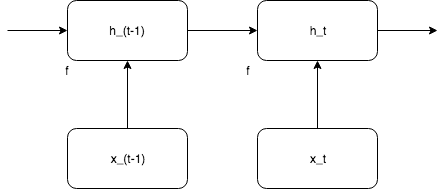
\includegraphics[width=9cm, height=3cm]{figures/rnnWithNoOutputs}
  \caption{A simple recurrent neural network}
  \label{f:rnnWithNoOutputs}
\end{figure}



Despite the fitness of applying RNNs to sequential data, the vanishing problem exists. Vanishing means the gradients become smaller and smaller as the network goes forward. When this happens, the networks are learning slowly or even stop learning. The main solution to the vanishing problem is using a more complex learning unit. In 1997, hochreiter invented Long Short Term Memory (LSTM) cell \cite{hochreiter1997long} which decreases the vanishing problem. LSTM has one more memory cell to remember long term context and uses a forget gate, a input gate and a output gate to control how much information to flow into and out of the current unit. Aside from LSTM, Cho et al. invented Gated Recurrent Unit (GRU)\cite{cho2014learning} which has a simplified structure but similar function with LSTM.


In this project, I used LSTM and GRU equally as learning unit. Among various RNN structures, I mainly used two types. The first type is a RNN with recurrent connections between hidden states as shown in Figure \ref{f:rnnWithNoOutputs}. The sequence of  states are needed. The second type is also a RNN with recurrent connections between hidden states. However, the last state is needed.

\section{Bidirectional Recurrent Neural Networks}

The RNNs in Section \ref{sect:rnn}
iterate from left to right. As such, the $h_t$ only contains context information from $x_1$ to $x_t$, but does not contain context information from $x_{t+1}$ to the end. However, in most sequence-to-sequence tasks, $h_t$ should contain the information of the whole sequence. Bidirectional RNNs make this possible. In a bidirectional RNN, one cell rolls from left to right, and another cell rolls from right to left. As illustrated in Figure \ref{f:bidirectionalRnn}, at time t, using both $h_t$ and $g_t$ can get context information of the whole sequence.

\begin{figure}[htbp]\centering
  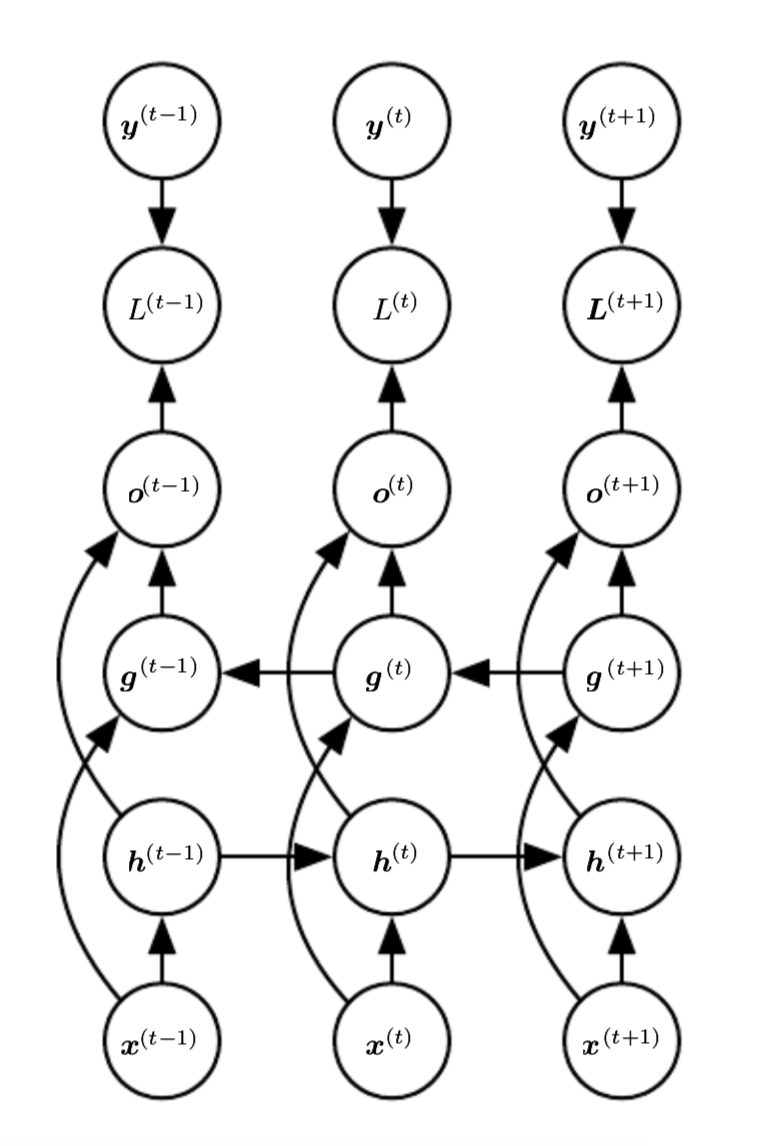
\includegraphics[width=8cm, height=5cm]{figures/bidirectionalRnn.png}
  \caption{A simple bidirectional recurrent neural network}
  \label{f:bidirectionalRnn}
\end{figure}

In this project, I used bidirectional RNNs in encoding part.

\section{Encoder-Decoder Sequence-to-Sequence Architecture}

Sequence-to-sequence means the input to a model is a sequence and the output from the model is also a sequence. An encoder-decoder architecture can be applied to do this task. The process of understanding the input sequence is considered as encoding the input sequence to some vectors $Crypto$. The process of generating output is considered as decoding the $Crypto$. Figure \ref{f:encoderDecoder} shows the concept of encoder-decoder sequence-to-sequence architecture . $x$ is the input, $h$ is the state in encoding process, $y$ is the output, and $g$ is the state of decoding process.

\begin{figure}[htbp]\centering
  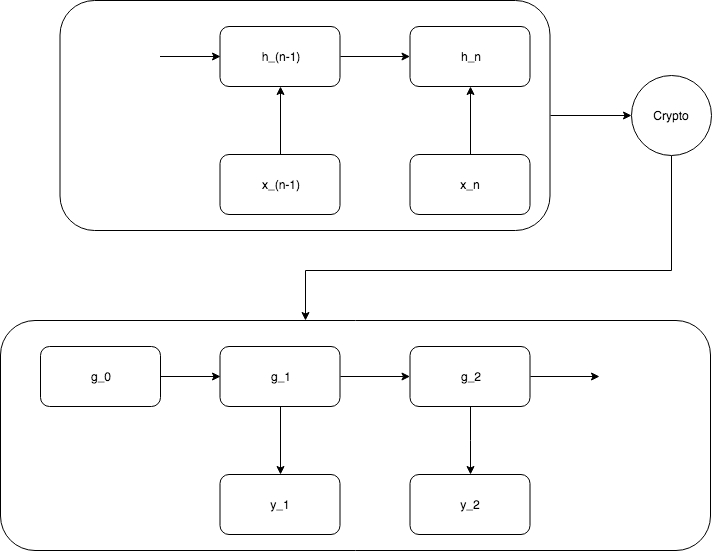
\includegraphics[width=10cm, height=7cm]{figures/encoderDecoder.png}
  \caption{Concept of encoder-decoder sequence-to-sequence architecture}
  \label{f:encoderDecoder}
\end{figure}

The question answering task in this project is a sequence-to-sequence task. However, some additional techniques must be equipped to the basic architecture in Figure \ref{f:encoderDecoder}. Each input actually includes two sequences - a question and a passage. As such, in the encoding process, some method is required to make each passage aware of the corresponding question and encode the two together. The attention mechanism discussed in Section \ref{sect:attention} is one such method. At the same time, each output sequence is an answer which is represented by two indices for the input passage sequence. A special decoding technique called pointer network discussed in Section \ref{sect:pointerNet} is needed.

\section{Attention Mechanism}\label{sect:attention}

Attention mechanism was firstly came up with by Bahdanau et al. in the application of neural machine translation\cite{bahdanau2014neural}. In a neural machine translation task, an encoder-decoder sequence-to-sequence model encodes each input sentence to some vectors and decodes the vectors to a sentence in another language with the same content. The attention mechanism is used to enable the decoding process aware of the encoding states $h_1, ... h_n$. As shown in Figure \ref{f:attention}, $y$ is the output, $g$ is the state, and $c$ is the attention vector. We have
$$g_i =f(g_{i-1},y_{i-1},c_i).$$
The attention vector $c_i$ is produced by using $g_{i-1}$ to ``query'' the encoding states $h_1, ... h_n$ through
$$c_i = \sum _j {\alpha _{i,j} h_j}$$
$$\alpha _{i,j} = \exp{e_{i,j}} / \sum _j {\exp{e_{i,j}}}$$
$$e_{i,j} = attention(h_j, g_{i-1}).$$
An example of the $attention$ function is $e_{i,j} = tanh(W_h h_j + W_g g_{i-1} + b)$.


\begin{figure}[htbp]\centering
  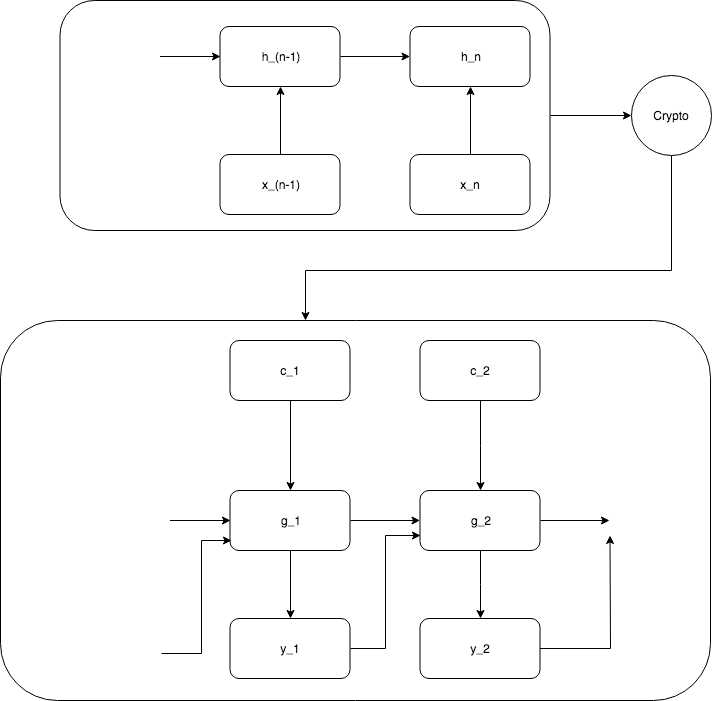
\includegraphics[width=8cm, height=8cm]{figures/attention}
  \caption{Attention mechanism in machine translation}
  \label{f:attention}
\end{figure}



Indeed, attention mechanism is a way to ``be aware of a sequence''. Since being aware of more context is a basic need of natural language processing tasks, it is reasonable to use attention mechanism in other tasks besides machine translation.

In this project, the passage is required to ``be aware of the question'' in encoding process. At the same time, the answer is required to ``be aware of the encoding states of passage and question''. The detailed formulas are given in Chapter \ref{chap:design}.




\section{Pointer Network}\label{sect:pointerNet}

Pointer network\cite{vinyals2015pointer} was invented by Vinyals et al. in 2015. Using pointer network enables decoder to output tokens from input sequence. Attention mechanism is used in pointer network. However, aside from getting an attention vector, the attention weight vector $\alpha$ is considered as a probability distribution which indicates how likely each token in input sequence is the current output. That is,
$$y_i = x_k$$
where
$$k = argmax_j(\alpha _{i,j}).$$
Note that compared with the machine translation architecture \ref{f:attention}, in pointer network, $y_i$ is not fed into the next decoding state.


\begin{figure}[htbp]\centering
  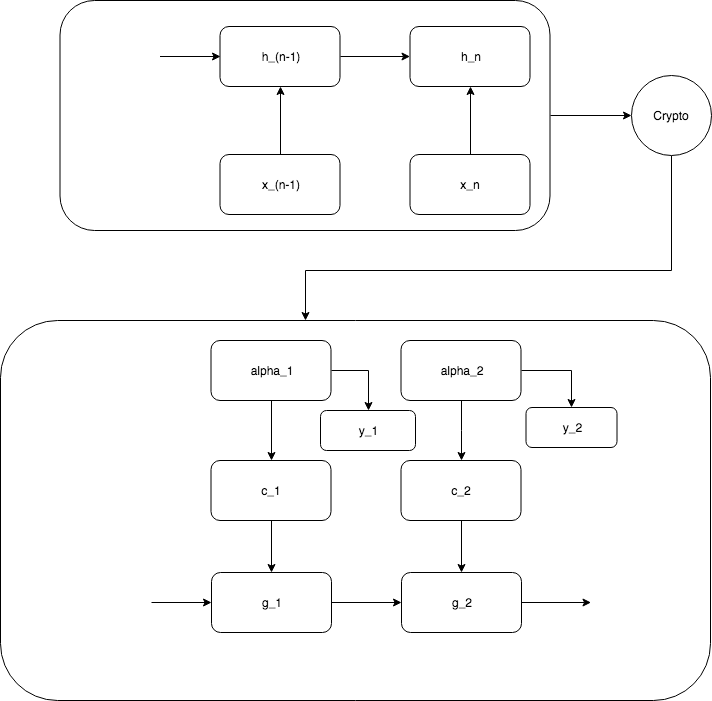
\includegraphics[width=8cm, height=8cm]{figures/pointerNetwork.png}
  \caption{Concept of pointer network}
  \label{f:pointerNetwork}
\end{figure}

In this project, pointer network was used in the decoding part of several models.


\chapter{Design}\label{chap:design}

In this chapter, I will explain the five models one by one. Recall that model one is the Match LSTM \& Answer Pointer model which has a typical encoder-decoder sequence-to-sequence recurrent network architecture designed by Wang and Jiang\cite{wang2016machine}. Model two, three, four and five are designed by making changes to model one.


\section{Model One}

Wang and Jiang  proposed an encoder-decoder sequence-to-sequence architecture for the question answering task on SQuAD dataset \cite{wang2016machine}. Each instance of training data includes one passage, one question and one answer. The passage is a sequence of tokens, the question is a sequence of tokens, and the answer is a sequence of two indices indicating the start and end positions in passage. Recall that each answer is part of the corresponding passage in SQuAD.

Before feeding training data into the model, tokens in passages and questions are vectorized to word feature vectors. As such, one pre-trained word feature vector matrix is an additional dataset required.

The vectorized training data is fed into the encoder. The encoder includes two layers - the preprocessing layer and the bidirectional match LSTM layer. In the preprossing layer, a LSTM runs over each passage word feature vector sequence and outputs a sequence of LSTM states. The same LSTM is used to encode each question word feature vector sequence to a sequence of LSTM states.

$$H^p = \overrightarrow{LSTM}(P)$$
$$H^q = \overrightarrow{LSTM}(Q)$$

where

 $$P\in R^{d \times p}: passage$$
 $$Q\in R^{d \times q}: question$$
 $$H^p\in R^{l \times p}: encoded\ passage$$
 $$H^q\in R^{l \times q}: encoded\ question$$
 $$p: length \ of\ passage$$
 $$q: length\ of\ question$$
 $$l: dimension\ of\ LSTM\ states$$
 $$d: dimension\ of\ word\ feature\ vector$$

In the bidirectional match LSTM layer, a LSTM equipped with passage-question attention, which is called match LSTM, is used to encode each sequence of passage states and the corresponding sequence of question states together to a sequence of match LSTM states. To be specific,

$$\overrightarrow{G} = tanh(W^qH^q + (W^p{h_i}^p + W^r\overrightarrow{{h_{i-1}}^r} + b^p) \otimes e_q)$$
$$\overrightarrow{\alpha _i} = softmax(w^t\overrightarrow{G_i} + b \otimes e_q)$$


where

$$W^q, W^p, W^r\in R^{l \times l} $$
$$b_p, w\in R^{l}  $$
$$b \in R $$
$${{h_{i}}pr}\in R^{l}: one\ column\ of\ H^p  $$

and

\[ \overrightarrow{z_i} =
\begin{bmatrix}
{h_i}^p \\
H^q\overrightarrow{ {\alpha _i}}^T \\
\end{bmatrix}
\in R^{2l}
\]
$$\overrightarrow{{h_i}^r} = \overrightarrow{LSTM}(\overrightarrow{z_i}, \overrightarrow{{h_{i-1}}^r}).$$

After iterating between getting attention weight vector $\overrightarrow{\alpha _i}$ and getting match LSTM state ${{h_{i}}^r}$ $p$ times, we get $[{{h_{1}}^r}, ..., {{h_{p}}^r}]$. Concatenate them to get

$$\overrightarrow{H^r} = [{{h_{1}}^r}, ..., {{h_{p}}^r}] \in R^{l \times p}.$$

Then go over $H^p$ from right to left to get $\overleftarrow{H^r}$. Concatenate $\overrightarrow{H^r}$ and $\overleftarrow{H^r}$ to get the final output of encoding process

\[ H^r =
\begin{bmatrix}
\overrightarrow{H^r} \\
\overleftarrow{H^r} \\
\end{bmatrix}
\in R^{2l \times p}.
\]

The decoding process includes only one layer - the answer pointer layer. This layer is motivated by the pointer network. Wang and Jiang proposed two ways to design this layer. Here I only explain the boundary way. In this way, each output of the decoding process includes two probability distributions. The first probability distribution tells how likely each token in passage to be the start of the answer. The second probability distribution tells how likely each token in passage to be the end of the answer. To be specific,

$$F_k = tahn(VH^r + (W^a{h^a_{k-1}} +  b^a) \otimes e_p)$$
$$\beta _k = softmax(v^tF_k + c \otimes e_p)$$


where
$$V \in R^{l \times 2l}$$
$$W^a\in R^{l \times l} $$
$$b_a, v\in R^{l}  $$
$$c \in R $$
$${h_{k-1}}^a\in R^{l}: ith\ state\ of\ answer\ LSTM  $$

and answer LSTM is


$${h_k}^a = LSTM(H^r\beta _k^T, h_{k-1}^a)$$

By iterating between the attention mechanism and the answer LSTM two times, we could get the output of the decoding process - $\beta _0$ and $\beta _1$.


Now we can get the loss function. Let $a_s$ denote the ground truth start index of the answer and $a_e$ denote the ground truth end index, we have

$$p(a|H^r) = p(a_s|H_r)p(a_r|H_r)=\beta _{0, a_s} \times \beta_{1, a_e}$$

where $$\beta_{k, j} = jth\ token\ of\ \beta _k$$

To train the model, the loss function

$$J(\theta) = -\frac{1}{N}\sum_{i=1}^{N} \log{p(a^n|H^r)} $$

is minimized.

\section{Model Two} \label{sect:change_0}

The difference from model two and model one is in the decoding process. In model two,
$${h_k}^a = H^r\beta _{k}^T.$$
That is, instead of the current state of answer LSTM, the previous attention vector is used to query the current attention weight vector.

\section{Model Three}

The difference between model three and model two is that in model three the $W^r\overrightarrow{{h_{i-1}}^r}$ in the bidirectional match LSTM layer is removed. This modification aims at checking whether $\overrightarrow{{h_{i-1}}^r}$ carries some redundant context information. After this change,


$$\overrightarrow{G} = tanh(W^qH^q + (W^p{h_i}^p + b^p) \otimes e_q)$$


\section{Model Four}

The difference between model four and model two is that in model four the the preprocessing layer is removed. This modification aims at checking whether the preprocessing layer carries some redundant context information.

\section{Model Five}

The difference between model five and model two is that in model five both the preprocessing layer and $W^r\overrightarrow{{h_{i-1}}^r}$ in the bidirectional match LSTM layer are removed. This aims at checking whether context information carried by both is included in some other parts of model two.

\chapter{Implementation}

\section{Adjusting Models for Batch Training}\label{sect:padding}

When training a model, all of the training data is fed into the model to update the parameters. In one specific model, the number of times to iterate the encoding process is fixed. However, different passages have different lengths and different questions also have different lengths. As such, adjusting all passages to a same length and adjusting all questions to another same length are necessary.

For sequences longer than a fixed length, a part of the sentence is cut out. For sequences shorter than a fixed length, a faking pad token is used to pad them. In practice, each passage is adjusted to $passage\_padding\_length$ and is paired with a mask vector $passage\_mask$ which has size $passage\_padding\_length$. Each question is adjusted to $question\_padding\_length$ and paired with a mask vector $question\_mask$ which has size $question\_padding\_length$. Each entry of mask vector is either zero or one. Zero indicates that the current token does not exist in the original sequence. One indicates the opposite.

When implementing a model, every effort is made to prevent the model from distracted tokens that do not exist. This makes the model in implementation different from the theoretical one. Take model one as an example. In the preprocessing layer, after getting a sequence of states, the mask vector is used to reset the values of positions that do not exist to zero in an additional step
$$H^p = H^p \circ (passage\_mask \otimes l)$$
$$H^q = H^q \circ (question\_mask \otimes l).$$
In the match LSTM layer, the attention weights of positions that do not exist are also set to zero in an additional step
$$\overrightarrow{\alpha _i} = softmax( (w^t\overrightarrow{G_i} + b \otimes e_q) ) \circ question\_mask .$$
Similar to the preprocessing layer, we have
$$H_r = H_r \circ (passage\_mask \otimes 2l).$$
In the answer pointer layer, similar to the match LSTM layer, we have
$$\beta _k = softmax( (v^tF_k + c \otimes e_p) ) \circ passage\_mask.$$


\section{Tensorflow Graphs}

Tensorflow is an open source machine learning framework. The central idea of Tensorflow is describing a complex numeric computation as a graph.  {\tt Variables} are ``trainable'' nodes.  {\tt Placeholders} are nodes whose values are fed in run time. Taking model one as an example,  {\tt Variables} should be used to represent all the parameters of the encoding and decoding layers and {\tt Placeholders} should be used to represent passages, questions, and answers. To train a graph, some APIs of Tensorflow are called to get a train operation. Then the training data is fed through {\tt Placeholders} to run the train operation. When the train operation is run, the {\tt Variables} are updated.

\begin{figure}[htbp]\centering
  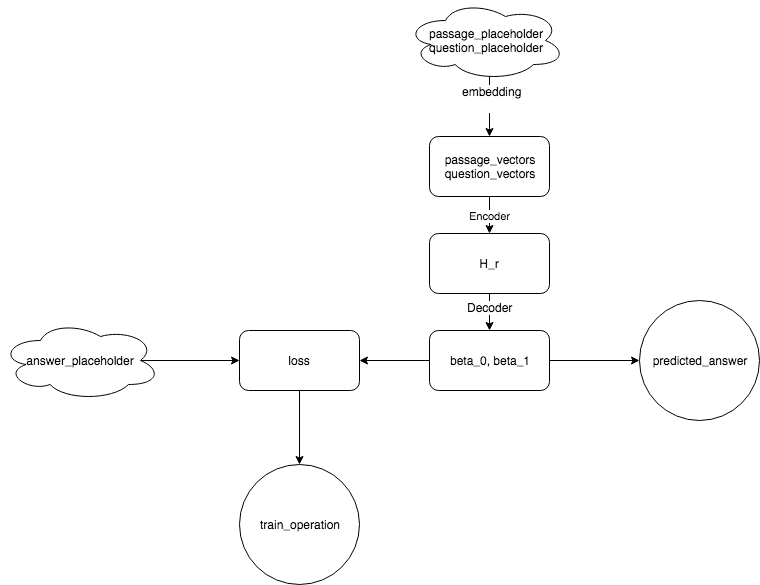
\includegraphics[width=12cm, height=12cm]{figures/tf_graph.png}
  \caption{Concept of the Tensorflow graphs used in this project}
  \label{f:tf_graph}
\end{figure}

Figure \ref{f:tf_graph} describes the concept of the Tensorflow graphs for five different models used in this project. The cloud shapes represent the {\tt Placeholders}. The {\tt Variables} are included in {\tt Encoder} and {\tt Decoder}. The rectangles represent nodes in the calculation process. The circles represent the final outputs used in training or testing.

Here is how to build the graph. In the embedding step, the model transforms word tokens into word feature vectors using a given word feature vector matrix. This matrix is part of the graph and is constant. The {\tt Encoder} encodes passage word feature vectors and question feature vectors to $H^r$. The {\tt Decoder} decodes $H^r$ to two probability distributions $\beta _0$ and $\beta _1$. Recall that $\beta _0$ tells how likely each token in a passage is the start of the answer and $\beta _1$ tells how likely each token in a passage is the end of the answer. The loss is calculated using $\beta _0$, $\beta _1$ and ground truth answers fed through answer {\tt Placeholders}. From the loss, a train operation is calculated.

Here is how the run time works. In training and validation process, the passages, questions and answers are fed into the graph. Running the train operation with data fed into through {\tt Placeholders} will update all the {\tt Variables}. In testing process, only passages and questions are fed into the graph. The predicted answers are determined from $\beta _0$ and $\beta _1$.






\section{Implementation Pipeline}

For a specific model, in the train and validation process, some Tensorflow graphs that have same structure but different values for {\tt Variables} are saved. The validation loss is used to choose the best graph. Then the best graph is used to do testing.

\begin{figure}[htbp]\centering
  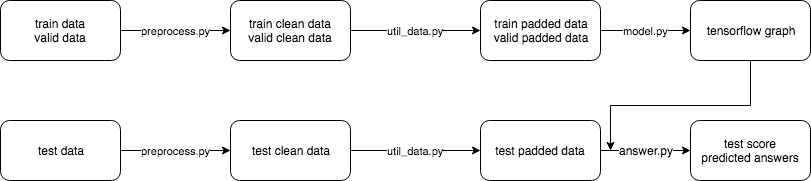
\includegraphics[width=11cm, height=3cm]{figures/pipeline.png}
  \caption{Implementation pipelines}
  \label{f:pipeline}
\end{figure}


\chapter{Experiments}
\section{Data}
The Stanford Question Answering Dataset (SQuAD) is used to do experiments. The GloVe word feature vectors\cite{pennington2014glove} are used to initialize words.

In the first step, a Python natural language processing library {\tt nltk} is used to tokenize raw data into passage word token sequences, question word token sequences and answer spans. Each answer span includes a start index and an end index. In total, our training set contains 78,839 instances, our validation set contains 8,760 instances, and our test set contains 10,570 instances.

\begin{table}[htbp]\centering
  \caption{Data sets}
  \label{tab:dataset}
  \begin{tabular}{|r|l|} \hline
    Set Name & Number of Instances \\ \hline\hline
    Train & \ 78,839 \\
    Validation & \ 8,760 \\
    Test & \ 10,570 \\ \hline
  \end{tabular}
\end{table}

The vocabulary is then made from the word token sequences from the training set and validation set. After the vocabulary is made, each word token is turned into its corresponding index in the vocabulary. Two special indices are used to represent the unknown token and the padding token. Before feeding index sequences into the Tensorflow graph, the index sequences are padded to fixed lengths, as mentioned in Section \ref{sect:padding}. The whole training data set is then split into mini batches to support stochastic gradient decent.

After the vocabulary is made, a smaller word feature vector matrix is made from the original GloVe word feature vectors. The smaller word feature vector matrix only includes vectors of words in the vocabulary. The unknown token is assigned an average of all the vectors of known tokens. The padding token is assigned a zero vector. The index of each token in the smaller word feature vector matrix is same as that in the vocabulary.

\begin{figure}[htbp]\centering
  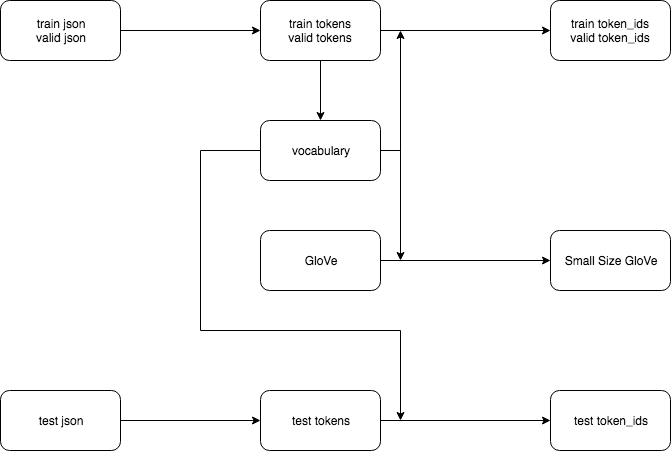
\includegraphics[width=12cm, height=9cm]{figures/data.png}
  \caption{Data pipelines}
  \label{f:data}
\end{figure}




\section{Settings}

Figure \ref{f:passage_length} shows the distribution of passage lengths. Figure \ref{f:question_length} shows the distribution of question lengths. Based on the distributions, 400 is set as $passage\_padding\_length$ and 30 is set as $question\_padding\_length$. We use the GloVe word feature vectors with size 100. The size of the LSTM state in the preprocessing layer, which is $l$ in theoretical model, is set at 64. The regularization scale of L2-regularization is set at 0.001. The batch size is set at 32. The adam optimizer is set using the default settings of Tensorflow. The normalization boundary to clip gradients is set at 5. 200 sample instances from training set are used to estimate training accuracy. 200 sample instances from validation set are used to estimate validation accuracy. The learning rate is selected through several experiments shown in Figure \ref{f:lr}. Based on these experiments, the learning rate is set at 0.002.

\begin{figure}[htbp]\centering
  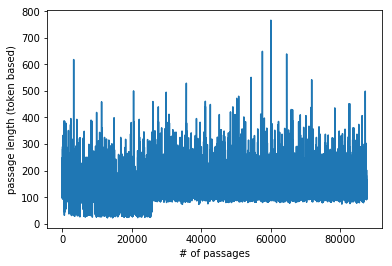
\includegraphics[width=10cm, height=7cm]{figures/passage_length.png}
  \caption{Distribution of passage lengths}
  \label{f:passage_length}
\end{figure}

\begin{figure}[htbp]\centering
  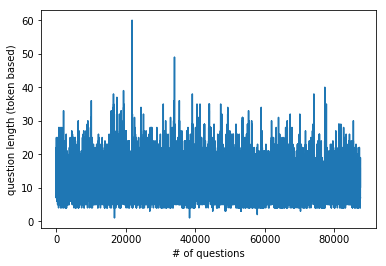
\includegraphics[width=10cm, height=7cm]{figures/question_length.png}
  \caption{Distribution of question lengths}
  \label{f:question_length}
\end{figure}

\begin{figure}[htbp]\centering
  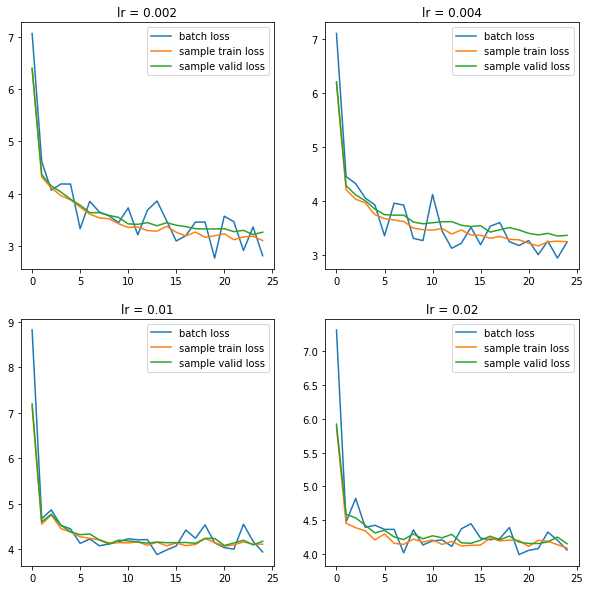
\includegraphics[width=12cm, height=12cm]{figures/lr.png}
  \caption{Performance of different learning rates}
  \label{f:lr}
\end{figure}

\begin{table}[htbp]\centering
  \caption{Experimental settings}
  \label{tab:settings}
  \begin{tabular}{|r|l|} \hline
    Hyperparameter Name& Value \\ \hline\hline
    Word Feature Vector Dimension (d) & \ 100 \\
    Hidden State Size (l) & \ 64 \\
    L2\_regularization Scale & \ 10570\\
    Hidden State Size (l) & \ 64\\
    Batch Size & \ 64\\
    Passage Length & \ 400\\
    Question Length & \ 30\\
    Clip Norm & \ 5\\
    Learning Rate & \ 0.002 \\ \hline
  \end{tabular}
\end{table}

F1 score and exact match score are used to evaluate the performance of each model. F1 treats a predicted answer and a ground truth as bag of words and calculate a harmonic average of precision and recall; exact match measures the percentage of predictions and ground truths that are exactly the same. The testing data contains several ground truth answers for one passage-question pair. The best score is chosen as the final score.

A machine that has Tesla K80 12 GB Memory, 61 GB RAM and 100 GB SSD is used to train the models.

\section{Results}
\subsection{Training Process}

Figure \ref{f:mlap}, \ref{f:baseline_change0}, \ref{f:baseline_change1}, \ref{f:baseline_change2} and \ref{f:baseline_change3} show the training process of five different models. One epoch contains roughly 25 * 100 mini batches. The training loss and training scores are calculated every 100 mini batches using the 200 sample instances from training set. We do the same for validation loss and validation scores. Training one epoch takes roughly 100 minutes. A thorough training of each model requires around 10 epochs and takes around 17 hours.

As indicated by Figure \ref{f:mlap}, model one converges after three epochs. The training F1 score converges to around 0.5, the training exact match score converges to around 0.35, the validation F1 score converges to around 0.3, and the validation exact match score converges to around 0.2.

As indicated by Figure \ref{f:baseline_change0}, model two keeps learning in 10 epochs. The training F1 score converges to around 0.6, the training exact match score converges to around 0.5, the validation F1 score converges to around 0.4, and the validation exact match score converges to around 0.3.

As indicated by Figure \ref{f:baseline_change1}, model three converges after 10 epochs. The training F1 score converges to around 0.65, the training exact match score converges to around 0.45, the validation F1 score converges to around 0.4, and the validation exact match score converges to around 0.3.

As indicated by Figure \ref{f:baseline_change2}, model four converges after four epochs. The training F1 score converges to around 0.6, the training exact match score converges to around 0.4, the validation F1 score converges to around 0.4, and the validation exact match score converges to around 0.2.

As indicated by Figure \ref{f:baseline_change3}, model five keeps learning in the 10 epochs. The training F1 score converges to around 0.5, the training exact match score converges to around 0.35, the validation F1 score converges to around 0.3, and the validation exact match score converges to around 0.2.

\begin{figure}[htbp]\centering
  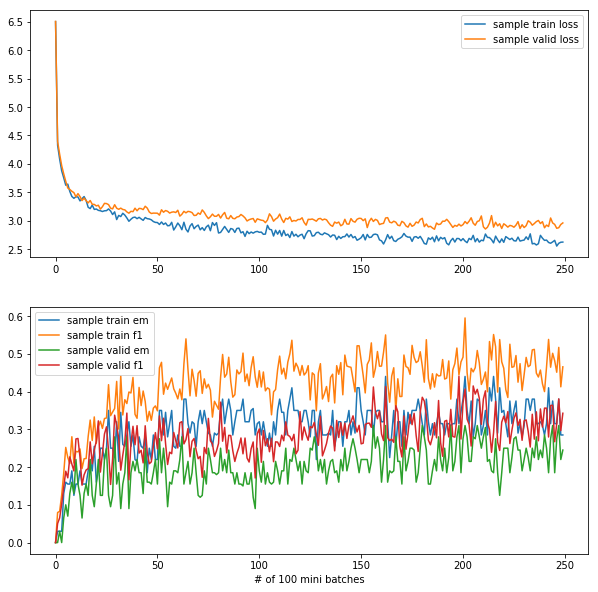
\includegraphics[width=12cm, height=12cm]{figures/match_corrected.png}
  \caption{Training process of model One}
  \label{f:mlap}
\end{figure}

\begin{figure}[htbp]\centering
  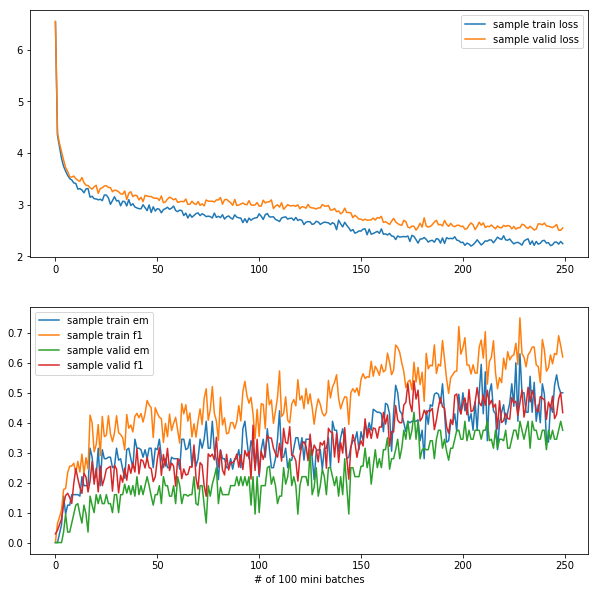
\includegraphics[width=12cm, height=12cm]{figures/match_baseline.png}
  \caption{Training process of model Two}
  \label{f:baseline_change0}
\end{figure}

\begin{figure}[htbp]\centering
  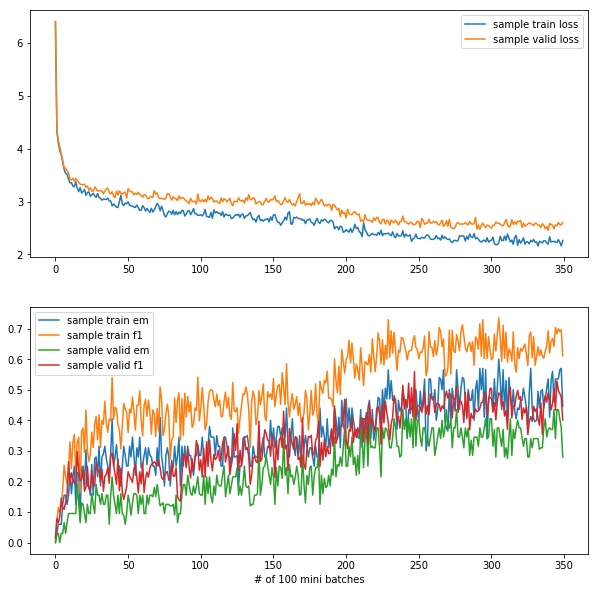
\includegraphics[width=12cm, height=12cm]{figures/match_change1.png}
  \caption{Training process of model Three}
  \label{f:baseline_change1}
\end{figure}

\begin{figure}[htbp]\centering
  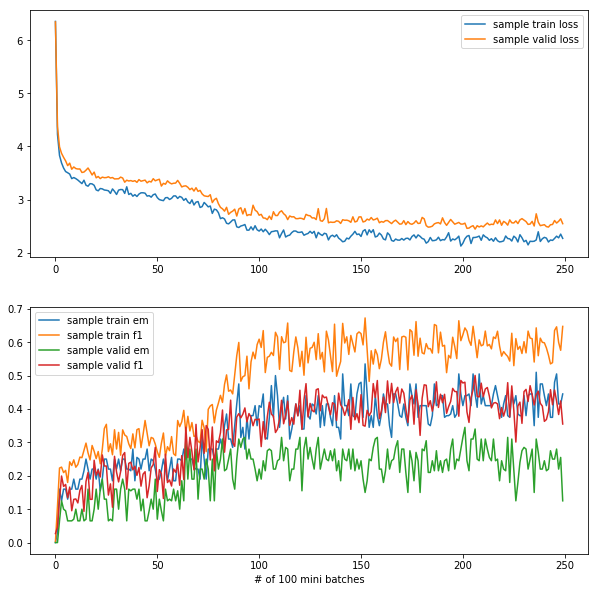
\includegraphics[width=12cm, height=12cm]{figures/match_change2.png}
  \caption{Training process of model Four}
  \label{f:baseline_change2}
\end{figure}

\begin{figure}[htbp]\centering
  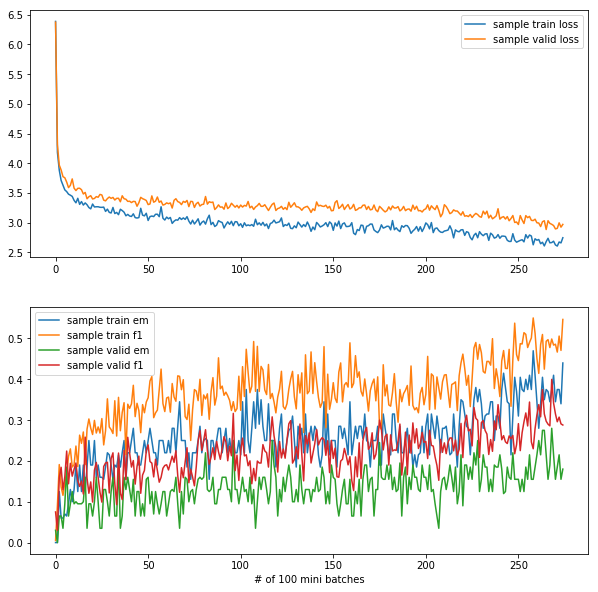
\includegraphics[width=12cm, height=12cm]{figures/match_change3.png}
  \caption{Training process of model Five}
  \label{f:baseline_change3}
\end{figure}

\subsection{Testing Results}

\begin{table}[htbp]\centering
  \caption{Testing results}
  \label{tab:test_results}
  \begin{tabular}{|c|c|c|}
    \hline
    Model& Test Exact Match & Test F1 \\
    \hline\hline
    Model One & \ 23.4 &\ 33.6 \\
    Model Two & \ 33.0 &\ 45.8 \\
    Model Three & \ 33.0 &\ 46.2 \\
    Model Four & \ 33.0 &\ 45.6 \\
    Model Five & \ 24.3 &\ 33.9 \\
    \hline
  \end{tabular}
\end{table}

Table \ref{tab:test_results} shows the testing results of all models. Model one gets F1 score 33.6 and exact match score 23.4. This does not reproduce the F1 score 71.2 and the exact match score 61.1 in the reference paper\cite{wang2016machine}. Model two, three and four behave similarly with F1 score around 46 and exact match score around 33. Model five behaves worse than the other three experiments with F1 score 33.9 and exact match score 24.3.




\section{Analysis}

Comparing testing results of model one with that of the original paper, the difference is quite surprising. To find out why my implementation does not reproduce the results of the original paper, further debugging and parameter tuning are needed.

Comparing the testing results of model two and model one, the scores of model two are better. As mentioned in Section \ref{sect:change_0}, model two uses previous attention vector to query the current attention weight vector. However, model one uses the current answer LSTM state to query the attention weight vector. The answer LSTM state is produced by applying a non-linear transformation on the attention vector. It turns out not including the non-linear transformation gives better results.

Model two, three and four behave similarly. This means removing either the preprocessing layer or the $h_r$ in the bidirectional match LSTM layer does not decrease test results. A reasonable guess is the two parts provide duplicate context information.

Model five performs worse than model two, three and four. This means removing both the preprocessing layer and the $h_r$ in the bidirectional match LSTM layer decreases testing results. A reasonable guess is the context information provided by these two parts is not provided in other parts of model one. As such, one of the two must be kept.





\chapter{Conclusion}

This project presented a thorough implementation of a question answering system. Five different models were tried and several interesting observations were found. Further work is required to find out why model one failed to reproduce the testing results of the reference paper.



% if you want to keep macros or chapters in separate files
% you can do that and include them with \input like this:

%\input macros.tex
%\input ch1.tex
%\input ch2.tex


%%%%%%%%%%%%%%%%%%%%%%%%%%%%%%%%%%%%%%%%%%%%%%%%%%%%%%%%%%%%%%%%%%%
%%%%%%%%%%%%%%%%%%%%%%%  Bibliography %%%%%%%%%%%%%%%%%%%%%%%%%%%%%
%%%%%%%%%%%%%%%%%%%%%%%%%%%%%%%%%%%%%%%%%%%%%%%%%%%%%%%%%%%%%%%%%%%

\bibliographystyle{amsalpha}	% or "siam", or "alpha", or "abbrv"
				% see other styles in
				% texmf/bibtex/bst

%\nocite{*}		% uncomment to list all refs in database,
			% cited or not.

\bibliography{refs}		% assumes bib database in "refs.bib"

%%%%%%%%%%%%%%%%%%%%%%%%%%%%%%%%%%%%%%%%%%%%%%%%%%%%%%%%%%%%%%%%%%%
%%%%%%%%%%%%%%%%%%%%%%%%  Appendices %%%%%%%%%%%%%%%%%%%%%%%%%%%%%%
%%%%%%%%%%%%%%%%%%%%%%%%%%%%%%%%%%%%%%%%%%%%%%%%%%%%%%%%%%%%%%%%%%%

% \appendix	% don't forget this line if you have appendices!

% \chapter{Gratuitous Appendix}
% Nothing to see here.

% %\input appA.tex


%%%%%%%%%%%%%%%%%%%%%%%%%%%%%%%%%%%%%%%%%%%%%%%%%%%%%%%%%%%%%%%%%%%
%%%%%%%%%%%%%%%%%%%%%%%%   THE END   %%%%%%%%%%%%%%%%%%%%%%%%%%%%%%
%%%%%%%%%%%%%%%%%%%%%%%%%%%%%%%%%%%%%%%%%%%%%%%%%%%%%%%%%%%%%%%%%%%

\end{document}
